%%%%%%%%%%%%%%%%%%%%%%%%%%%%%%%%%%%%%%%%%%%%%%%%%%%%%%%%%%%%%%%%%%%%%%%%%%
%Author:																 %
%-------																 %
%Yannis Baehni at University of Zurich									 %
%baehni.yannis@uzh.ch													 %
%																		 %
%Version log:															 %
%------------															 %
%06/02/16 . Basic structure												 %
%04/08/16 . Layout changes including section, contents, abstract.		 %
%05/11/16 . Simon, name changes%
%%%%%%%%%%%%%%%%%%%%%%%%%%%%%%%%%%%%%%%%%%%%%%%%%%%%%%%%%%%%%%%%%%%%%%%%%%

%Page Setup
\documentclass[
	11pt, 
	oneside, 
	a4paper,
	reqno,
	final
]{amsart}

\usepackage[
	left = 3cm, 
	right = 3cm, 
	top = 3cm, 
	bottom = 3cm
]{geometry}

%Headers and footers
\usepackage{fancyhdr}
	\pagestyle{fancy}
	%Clear fields
	\fancyhf{}
	%Header right
	\fancyhead[R]{
		\footnotesize
		Simon Gr\"uning\\
		\href{mailto:simon.gruening@uzh.ch}{simon.gruening@uzh.ch}
	}
	%Header left
	\fancyhead[L]{
		\footnotesize
		MAT694 Seminar: Introduction to Harmonic Analysis\\
		HS16
	}
	%Page numbering in footer
	\fancyfoot[C]{\thepage}
	%Separation line header and footer
	\renewcommand{\headrulewidth}{0.4pt}
	%\renewcommand{\footrulewidth}{0.4pt}
	
	\setlength{\headheight}{19pt} 

%Title
\usepackage[foot]{amsaddr}
\usepackage{xspace}
\makeatletter
\def\@textbottom{\vskip \z@ \@plus 1pt}
\let\@texttop\relax
\usepackage{etoolbox}
\patchcmd{\abstract}{\scshape\abstractname}{\textbf{\abstractname}}{}{}

%Switching commands for different section formats
%Mainsectionsytle
\newcommand{\mainsectionstyle}{%
  	\renewcommand{\@secnumfont}{\bfseries}
  	\renewcommand\section{\@startsection{section}{1}%
    	\z@{.5\linespacing\@plus.7\linespacing}{-.5em}%
    	{\normalfont\bfseries}}%
	\renewcommand\subsection{\@startsection{subsection}{2}%
    	\z@{.5\linespacing\@plus.7\linespacing}{-.5em}%
    	{\normalfont\bfseries}}%
	\renewcommand\subsubsection{\@startsection{subsubsection}{3}%
    	\z@{.5\linespacing\@plus.7\linespacing}{-.5em}%
    	{\normalfont\bfseries}}%
}
\newcommand{\originalsectionstyle}{%
\def\@secnumfont{\bfseries}%\mdseries
\def\section{\@startsection{section}{1}%
  \z@{.7\linespacing\@plus\linespacing}{.5\linespacing}%
  {\normalfont\bfseries\centering}}
}
%Formatting title of TOC
\renewcommand{\contentsnamefont}{\bfseries}
%Table of Contents
\setcounter{tocdepth}{3}

% Add bold to \section titles in ToC and remove . after numbers
\renewcommand{\tocsection}[3]{%
  \indentlabel{\@ifnotempty{#2}{\bfseries\ignorespaces#1 #2\quad}}\bfseries#3}
% Remove . after numbers in \subsection
\renewcommand{\tocsubsection}[3]{%
  \indentlabel{\@ifnotempty{#2}{\ignorespaces#1 #2\quad}}#3}
\let\tocsubsubsection\tocsubsection% Update for \subsubsection
%...

\newcommand\@dotsep{4.5}
\def\@tocline#1#2#3#4#5#6#7{\relax
  \ifnum #1>\c@tocdepth % then omit
  \else
    \par \addpenalty\@secpenalty\addvspace{#2}%
    \begingroup \hyphenpenalty\@M
    \@ifempty{#4}{%
      \@tempdima\csname r@tocindent\number#1\endcsname\relax
    }{%
      \@tempdima#4\relax
    }%
    \parindent\z@ \leftskip#3\relax \advance\leftskip\@tempdima\relax
    \rightskip\@pnumwidth plus1em \parfillskip-\@pnumwidth
    #5\leavevmode\hskip-\@tempdima{#6}\nobreak
    \leaders\hbox{$\m@th\mkern \@dotsep mu\hbox{.}\mkern \@dotsep mu$}\hfill
    \nobreak
    \hbox to\@pnumwidth{\@tocpagenum{\ifnum#1=1\bfseries\fi#7}}\par% <-- \bfseries for \section page
    \nobreak
    \endgroup
  \fi}
\AtBeginDocument{%
\expandafter\renewcommand\csname r@tocindent0\endcsname{0pt}
}
\def\l@subsection{\@tocline{2}{0pt}{2.5pc}{5pc}{}}
\def\l@subsubsection{\@tocline{2}{0pt}{4.5pc}{5pc}{}}
\makeatother

\advance\footskip0.4cm
\textheight=54pc    %a4paper
\textheight=50.5pc %letterpaper
\advance\textheight-0.4cm
\calclayout

%Font settings
%\usepackage{anyfontsize}
%Footnote settings
%\usepackage{mathptmx}
\usepackage{footmisc}
%	\renewcommand*{\thefootnote}{\fnsymbol{footnote}}

%Further math environments
%Further math fonts (loads amsfonts implicitely)
\usepackage{amssymb}
%Redefinition of \text
%\usepackage{amstext}
\usepackage{upref}
%Graphics
%\usepackage{graphicx}
%\usepackage{caption}
%\usepackage{subcaption}
%Frames
\usepackage{mdframed}
\allowdisplaybreaks
%\usepackage{interval}
\newcommand{\toup}{%
  \mathrel{\nonscript\mkern-1.2mu\mkern1.2mu{\uparrow}}%
}
\newcommand{\todown}{%
  \mathrel{\nonscript\mkern-1.2mu\mkern1.2mu{\downarrow}}%
}
\AtBeginDocument{\renewcommand*\d{\mathop{}\!\mathrm{d}}}
\renewcommand{\Re}{\operatorname{Re}}
\renewcommand{\Im}{\operatorname{Im}}
\DeclareMathOperator\Log{Log}
\DeclareMathOperator\Arg{Arg}
\DeclareMathOperator\sech{sech}
%\usepackage{hhline}
%\usepackage{booktabs} 
%\usepackage{array}
%\usepackage{xfrac} 
%\everymath{\displaystyle}
%Enumerate
\usepackage{tikz}
\usetikzlibrary{external}
\tikzexternalize % activate!
\usetikzlibrary{patterns}
\pgfdeclarepatternformonly{adjusted lines}{\pgfqpoint{-1pt}{-1pt}}{\pgfqpoint{40pt}{40pt}}{\pgfqpoint{39pt}{39pt}}%
{
  \pgfsetlinewidth{.8pt}
  \pgfpathmoveto{\pgfqpoint{0pt}{0pt}}
  \pgfpathlineto{\pgfqpoint{39.1pt}{39.1pt}}
  \pgfusepath{stroke}
}
\usepackage{enumitem} 
%\renewcommand{\labelitemi}{$\bullet$}
%\renewcommand{\labelitemii}{$\ast$}
%\renewcommand{\labelitemiii}{$\cdot$}
%\renewcommand{\labelitemiv}{$\circ$}
%Colors
%\usepackage{color}
%\usepackage[cmtip, all]{xy}
%Theorems
\newtheoremstyle{bold}              	 %Name
  {}                                     %Space above
  {}                                     %Space below
  {\itshape}		                     %Body font
  {}                                     %Indent amount
  {\scshape}                             %Theorem head font
  {.}                                    %Punctuation after theorem head
  { }                                    %Space after theorem head, ' ', 
  										 %	or \newline
  {} 
\theoremstyle{bold}
\newtheorem*{definition*}{Definition}
\newtheorem{definition}{Definition}[section]
\newtheorem*{lemma*}{Lemma}
\newtheorem{lemma}{Lemma}[section]
\newtheorem{Proof}{Proof}[section]
\newtheorem{proposition}{Proposition}[section]
\newtheorem{properties}{Properties}[section]
\newtheorem{corollary}{Corollary}[section]
\newtheorem*{theorem*}{Theorem}
\newtheorem{theorem}{Theorem}[section]
\newtheorem{example}{Example}[section]
\newtheorem*{remark*}{Remark}
\newtheorem{remark}{Remark}[section]
%German non-ASCII-Characters
%Graphics-Tool
%\usepackage{tikz}
%\usepackage{tikzscale}
%\usepackage{bbm}
%\usepackage{bera}
%Listing-Setup
%Bibliographie
\usepackage[backend=bibtex, style=alphabetic]{biblatex}
%\usepackage[babel, german = swiss]{csquotes}
\bibliography{Bibliography}
%PDF-Linking
%\usepackage[hyphens]{url}
\usepackage[bookmarksopen=true,bookmarksnumbered=true]{hyperref}
%\PassOptionsToPackage{hyphens}{url}\usepackage{hyperref}
\hypersetup{
  colorlinks   = true, %Colours links instead of ugly boxes
  urlcolor     = blue, %Colour for external hyperlinks
  linkcolor    = blue, %Colour of internal links
  citecolor    = blue %Colour of citations
}
%Weierstrass-P symbol for power set
\newcommand{\powerset}{\raisebox{.15\baselineskip}{\Large\ensuremath{\wp}}}

\begin{document}

\title{Convolution and Approximate Identities}
\author{Simon Gr\"uning}
\address[Simon Gr\"uning]{University of Zurich, R\"{a}mistrasse 71, 8006 Zurich}
\email[Simon Gr\"uning]{\href{mailto:simon.gruening@uzh.ch}{simon.gruening@uzh.ch}}



\maketitle
\addtocounter{section}{1}

\section{Examples of Topological Groups}



\begin{definition}
Topological Group
\end{definition}

\begin{definition}
Locally Compact
\end{definition}

\begin{definition}
Haar Measure
\end{definition}

	\begin{example}
	$\mathbb{R}^n, \mathbb{Z}^n, \mathbb{T}^n$
	\end{example}
	
\begin{example}
$dx/|x|$
\end{example}	
	
\begin{example}
Heisenberg Group $\mathbb{H}^n$
\end{example}	

	
\section{Convolution}

\begin{definition}
 Let $f,g \in L^1(G)$. Define the \textbf{convolution} $f*g$ by
\begin{equation}
 (f*g)(x) := \int_G f(y)g(y^{-1}x) d\lambda(y)
\end{equation}
\end{definition}

\begin{remark}
Note that on $\mathbb{R}^n$ with an additive structure (our preferred environment for later chapters), we will simply have:
\begin{equation*}
 (f*g)(x) = \int_{\mathbb{R}^n} f(y)g(x-y) dy
\end{equation*}
\end{remark}

\begin{example}
Let $G = \mathbb{R}$, 
\begin{equation}
f(x) = \begin{cases}
1 & -1 \leq x \leq 1 \\
0 & \text{else}
\end{cases}
\end{equation}
Then we calculate:
\begin{align*}
(f \ast f)(x) &= \int_\mathbb{R} f(y)f(x-y) d\lambda(y) \\
&= 
\begin{cases}
\displaystyle
\int_\mathbb{R} 0 d\lambda(y) & -1 \leq x \leq 1 \\
\displaystyle
\int_\mathbb{R} \chi_{\intcc{-1,1}\cap\intcc{x-1,x+1}}(x) d\lambda(x) & \text{else}
\end{cases} 
\end{align*}

Notice that the convolution operator has a natural smoothing effect on $f$, as it does on every function.

\end{example}

\begin{lemma}
Convolution is defined $\lambda$ almost everywhere. 
\end{lemma}

\begin{proof}To see this we take the $L_1$ norm on the definition to find it finite:
\begin{align*}
\tag{Apply Norm}
 \norm{(f \ast g)(x)}_{L^1} &= \int_G \abs{ \int_G f(y) g(y^{-1}x) d\lambda(y) } d\lambda(x) 
\\ 
\tag{Tri. Ineq.}
&\leq \int_G \int_G \abs[0]{f(y)} \abs[0]{g(y^{-1}x)} d\lambda(y) d\lambda(x) \\
 \tag{Fubini}
&=  \int_G \int_G \abs[0]{f(y)} \abs[0]{g(y^{-1}x)} d\lambda(x) d\lambda(y) \\
 \tag{Measure-Invariance}
&=  \int_G \abs[0]{f(y)} \int_G  \abs[0]{g(y^{-1}x)} d\lambda(x) d\lambda(y) \\
 \tag{Left Haar}
&=  \int_G \abs[0]{f(y)} \int_G  \abs[0]{g(x)} d\lambda(x) d\lambda(y) \\
 \tag{Def.}
 &= \norm{f}_{L^1} \norm{g}_{L^1} \\
 \tag{Def.}
 &< \infty
\end{align*}
\end{proof}

\begin{lemma}
\begin{equation*}
(f \ast g)(x) = \int_G f(xz)g(z^{-1}) d\lambda(z)
\end{equation*}
\end{lemma}

\begin{proof}
We perform a change of variables $z = x^{-1}y$:
\begin{align*}
(f \ast g)(x) &= \int_G f(y)g(y^{-1}x) d\lambda(y) \\
&= \int_G f(xx^{-1}y)g((yx^{-1})^{-1}) d\lambda(y) \\
\tag{Left Invariance}
&= \int_G f(xz)g(z^{-1}) d\lambda(x^{-1}y) \\
&= \int_G f(xz)g(z^{-1}) d\lambda(z) \\
\end{align*}
\end{proof}

\begin{proposition}

$\forall f,g,h \in L^1(G):$
\begin{enumerate}
\item
$f \ast (g \ast h) = (f \ast g) \ast h $
\item
$f \ast (g + h) = f \ast g + f \ast h \wedge (f+g) \ast h = f\ast h + f\ast g $
\end{enumerate}
Thus convolution is associative and distributive.
\end{proposition}

\begin{proof}
Associativity:
\begin{align*}
ZZZZZZZZZZ
\end{align*}
Distributivity:
\begin{align*}
f \ast (g + h) &= \int_G f(y) (g+h)(y^{-1}x)d\lambda(y)\\
&= \int_G f(y) (g(y^{-1}x)+h(y^{-1}x))d\lambda(y)\\
&= \int_G f(y)g(y^{-1}x)+f(y)h(y^{-1}x)d\lambda(y)\\
&= \int_G f(y)g(y^{-1}x) d\lambda(y) + \int_G f(y)h(y^{-1}x) d\lambda(y)\\
&= f \ast g + f \ast h
\end{align*}
The mirror statement follows analogously. 
\end{proof}

\begin{remark}
\begin{proof} Notice the following trivial equality:\begin{align*}
\norm{f}^{p/q}_{L^p} &= (( \int_G \abs{f(x)}^p d\lambda(x) )^{1/p} ) ^ {p/q} \\
&= (\int_G \abs{f(x)}^p d\lambda(x) )^{1/q}
\end{align*} \end{proof}
\end{remark}

\section{Basic Convolution Inequalities}

\begin{definition}
Define $ p' := p / (p-1) $. To maintain our desired property in infinity we also declare: $1 / \infty = 0$
\end{definition}

\begin{remark}
Notice then: $\frac{1}{p} + \frac{1}{p'} = \frac{1}{p} + \frac{p-1}{p} = \frac{p}{p} = 1$
\end{remark}

\begin{remark}
In the following proofs we often make use of this useful inequality without further explication, it allows us to manipulate inequalities without worrying about negatives:
\begin{align*}
f \ast g &= \int_G f(y)g(y^{-1}x) d\lambda(y) \\
&\leq \abs{ \int_G f(y)g(y^{-1}x) d\lambda(y) } \\
&\leq \int_G \abs[0]{f(y)}\abs[0]{g(y^{-1}x)} d\lambda(y) \\
&= \abs{f} \ast \abs{g}
\end{align*}
\end{remark}

What follows is akin to the triangle inequality for $L^p$ spaces.

\begin{theorem}
Minkowskis Inequality: Let $1 \leq p \leq \infty$, $f \in L^p (G)$, $g \in L^1(G)$ then it follows that: 
$g \ast f $exists $\lambda$-almost-everywhere and
$ \norm{g \ast f}_{L^p(G)} \leq \norm{g}_{L^1(G)} \norm{f}_{L^p(G)} $
\end{theorem}

\begin{proof}
First we shall inspect the easier case of $p=1$:
ZZZZZZprooofZZZZ


Similarly we may rid ourselves of the other easy case $p=\infty$:
ZZZZproofZZZZ

For $ 1 < p < \infty$, we must work a little harder. We have:
\begin{equation*}
(\abs{g} \ast \abs{f} )(x) = \int_G \abs{f(y^{-1}x)}\abs{g(y)} d\lambda(y)
\end{equation*}
We shall apply H\"olders inequality as follows ZZZ to recieve:
\begin{equation*}
(\abs{g} \ast \abs{f} )(x) \leq (\int_G \abs{f(y^{-1}x)}^p \abs{g(y)} d\lambda(y))^{1/p} (\int_G \abs{g(y)} d\lambda(y))^{1/p'}
\end{equation*}

Since we are insane ZZZZ we may take the $L^p$ norm on both sides while preserving the inequality.

\begin{align*}
\norm{\abs{g} \ast \abs{f}}_{L^p} &= () \\
&= blah
\end{align*}

\end{proof}

\begin{theorem}
Youngs Inequality
\end{theorem}


\begin{theorem}
Youngs Inequality for Weak Type Spaces
ouch proof
\end{theorem}

\section{Approximate Identities}

Approximation of dirac delta function , identity element of convolutions

\begin{definition}
An \textbf{approximate identity} (as $\varepsilon \rightarrow 0$) is a family of $L^1(G)$ functions $k_\varepsilon$ with the following three properties: 
\begin{enumerate}[label=(\roman*)]
\item There exists a constant $c > 0$ such that $\| k_\varepsilon \| _ {L^1(G)} \leqslant c$ for all $ \varepsilon > 0 $ . 
\item $ \int_G k_\varepsilon(x) d\lambda(x) = 1$ for all $\varepsilon > 0 $.
\item For any neighborhood $V$ of the identity element $e$ of the group G we have $ \int_{V^c} | k_\varepsilon(x) | d \lambda(x) \rightarrow 0  $ as $ \varepsilon \rightarrow 0 $ . 
\end{enumerate}
\end{definition}

\begin{theorem}
Any approximate identity has the following two properties:
\begin{enumerate}
\item $f \in L^p(G) \wedge 1 \leq p < \infty \implies \norm{k_\epsilon \ast f - f}_{L^p(G)} \to 0 $ as $ \epsilon \to 0$
\item $f \in L^\infty(G)$ uniformly continuous on $K \subset G \implies \norm{k_\epsilon \ast f - f}_{L^\infty(K)} \to 0$ as $\epsilon \to 0$ \\
Furthermore, if $f$ is bounded and continuous at $x \in G$ then
$ (k_\epsilon \ast )(x) \to f(x) $ as $\epsilon \to 0$ 
\end{enumerate}
\end{theorem}

\begin{proof}
Let us first prove the statement in finite $L^p$ spaces. We shall make use of the following equality:
\begin{align*}
\forall p \in \mathbb{N} : \abs{g(h^{-1}x) - g(x)}^p &\leq (\abs{g(h^{-1}x)}+\abs{g(x)})^p \\
&\leq (\esssup_x (\abs{g(h^{-1}x)} )+\esssup_x(\abs{g(x)}) )^p \\
&\leq (2\norm{g}_{L^\infty})^p
\end{align*}
Applying the Lebesgue Dominated Convergence theorem (*) we find:
\begin{align*}
\int_G \abs{g(h^{-1}x)-g(x)}^p d\lambda(x) \to 0 \text{ as } h \to e
\end{align*}
Where $e$ is the neutral element of $G$. In $\mathbb{R}^n$ this is simply $0$. We can approximate any $g \in L^p(G)$ with a continuous function $f$ with compact support. Thus the property still holds:
\begin{align*}
\int_G \abs{f(h^{-1}x)-f(x)}^p d\lambda(x) \to 0 \text{ as } h \to e
\end{align*}
However we can now say that since $f$ is continuous,
\begin{equation}
\delta > 0 : \exists V(e): h \in V(e) \implies \int_G \abs{f(h^{-1}x) - f(x)}^p d\lambda(x) < (\frac{\delta}{2})^p ( \frac{1}{c})
\end{equation}
Where $c*$, $V(e)$ is a neighborhood of $e$. We shall fix this neighborhood for later. We have picked the value on the right side for later convenience. As with most proofs in this area, we shall split the object of our analysis into two parts we can evaluate:
\begin{align*}
(k_\epsilon \ast f)(x) - f(x) &= \int_G (f(y^{-1}x)-f(x))k_\epsilon(y) d\lambda(y)
\end{align*}
We take $L^p$ norms on both sides. This preserves the equality since *.
\begin{align*}
\norm{(k_\epsilon \ast f)(x) - f(x)}_{L^p(G)} &= \norm{\int_G (f(y^{-1}x)-f(x))k_\epsilon(y) d\lambda(y)}_{L^p(G)} \\
&= (\int_G \abs{\int_G (f(y^{-1}x)-f(x))k_\epsilon(y) d\lambda(y)}^p d\lambda(x) )^{\frac{1}{p}}\\
&\leq (\int_G \int_G \abs{f(y^{-1}x)-f(x)}^p \abs{k_e(y)}  d\lambda(y) d\lambda(x) )^{\frac{1}{p}} \\
&= (\int_G \int_V \abs{f(y^{-1}x)-f(x)}^p \abs{k_e(y)} d\lambda(y) d\lambda(x) 
+ \int_G \int_{V^c} \abs{f(y^{-1}x)-f(x)}^p \abs{k_e(y)} d\lambda(y) d\lambda(x) )^{\frac{1}{p}}
\end{align*}
Where the inequality originates from Jensen's inequality *. Notice that we can now inspect on $V$ and $V^c$, we shall call the respective parts of the function $F_V$ and $F_{V^c}$ such that our last statement can be rewritten as $ ( F_V + F_{V_c} )^{\frac{1}{p}}$ for convenience. We now look at them individually. 

\begin{align*}
F_V &= \int_G \int_V \abs{f(y^{-1}x)-f(x)}^p \abs{k_e(y)} d\lambda(y) d\lambda(x)\\
&= \int_V \int_G \abs{f(y^{-1}x)-f(x)}^p \abs{k_e(y)} d\lambda(x) d\lambda(y)\\
&= \int_V \int_G \abs{f(y^{-1}x)-f(x)}^p  d\lambda(x) \abs{k_e(y)} d\lambda(y)\\
&\leq \int_V ( (\frac{\delta}{2})^p \frac{1}{c} ) \abs{k_e(y)} d\lambda(y)\\
&= ( (\frac{\delta}{2})^p \frac{1}{c} ) \int_V  \abs{k_e(y)} d\lambda(y)\\
&\leq ( (\frac{\delta}{2})^p \frac{1}{c} ) \int_G  \abs{k_e(y)} d\lambda(y)\\
&\leq ( (\frac{\delta}{2})^p \frac{1}{c} ) c\\
&= ( (\frac{\delta}{2})^p )\\
\end{align*}
Here we have used Fubini *, substituted our previously discovered upper bound, and used property $(i)$ intrinsic of any approximate identity, as defined. We bound the other half now:

\begin{align*}
F_{V^p} &= \int_G \int_{V^c} \abs{f(y^{-1}x)-f(x)}^p \abs{k_\epsilon(y)} d\lambda(y) d\lambda(x) \\
&= \int_{V^c} \int_{G} \abs{f(y^{-1}x)-f(x)}^p \abs{k_\epsilon(y)} d\lambda(x) d\lambda(y) \\
&= \int_{V^c} \norm{f(y^{-1}x)-f(x)}^p_{L^p} \abs{k_\epsilon(y)} d\lambda(x) d\lambda(y) \\
&\leq \int_{V^c} (\norm{f}^p_{L^p}+\norm{f}^p_{L^p}) \abs{k_\epsilon(y)} d\lambda(x) d\lambda(y) \\
&= \int_{V^c} (2\norm{f}^p_{L^p}) \abs{k_\epsilon(y)} d\lambda(x) d\lambda(y) \\
&= (2\norm{f}^p_{L^p}) \int_{V^c} \abs{k_\epsilon(y)} d\lambda(x) d\lambda(y) \\
&\leq (2\norm{f}^p_{L^p}) \int_{V^c} \abs{k_\epsilon(y)} d\lambda(x) d\lambda(y) \\
ZZZ \\
&\leq ( (\frac{\delta}{2})^p )
\end{align*}
Were we have once again used Fubini *, the definition of our norm, minkowski's *, and have choosen a correct neighborhood $V^c$... *. Putting our function back together we find:

\begin{align*}
(F_V + F_{V^c}) &\leq (\frac{\delta}{2})^p + (\frac{\delta}{2})^p ) ^{\frac{1}{p}}\\
&\leq (\frac{\delta}{2})+(\frac{\delta}{2}))\\
&= \delta\\
\end{align*}

Where the final inequality follows from the fact that $p \geq 1 \implies \frac{1}{p} \leq 1$ and Ex. 1.1.4 from the previous section. We have proven property $(1)$ of our theorem since the norm becomes arbitrarily small and thus converges to 0.

We shall no prove the case of $ p = \infty$. First we prepare some ingredients. We have required that f is bounded and uniformly continuous. Recall:

\begin{align*}
f \text{uniformly continuous} \implies \delta > 0 : \forall  V(e): \abs{f(y^{-1}x)-f(x)} < \frac{\delta}{2c}
\end{align*}

Furthermore from property $(iii)$ of an approximate identity we have:

\begin{align*}
\exists \epsilon_0 > 0 : \forall \epsilon \in (0,\epsilon_0): \int_{V^c} \abs{k_\epsilon(y)} d\lambda(y) \leq \frac{\delta}{2(\norm{f}_{L^\infty}+1)}
\end{align*}

Once more we shall split our normed function:

\begin{align*}
\norm{k_\epsilon \ast f -f}_{L^\infty}(G) &= \sup_{x\in G} \abs{(k_\epsilon \ast f)(x)-f(x)} \\
&= \sup_{x\in G} \abs{\int_G f(y^{-1}x)-f(x) k_\epsilon(y) d\lambda(y)}\\
&= \sup_{x\in G} \abs{\int_V f(y^{-1}x)-f(x) k_\epsilon(y) d\lambda(y) + \int_{V^c} f(y^{-1}x)-f(x) k_\epsilon(y) d\lambda(y)}\\
&\leq \sup_{x\in G} \abs{\int_V f(y^{-1}x)-f(x) k_\epsilon(y) d\lambda(y)} + \abs{\int_{V^c} f(y^{-1}x)-f(x) k_\epsilon(y) d\lambda(y)} \\
&\leq \sup_{x\in G} \abs{\int_V f(y^{-1}x)-f(x) k_\epsilon(y) d\lambda(y)} + \sup_{x\in G} \abs{\int_{V^c} f(y^{-1}x)-f(x) k_\epsilon(y) d\lambda(y)} \\
&\leq \sup_{x\in G} \int_V \abs{f(y^{-1}x)-f(x)}\abs{ k_\epsilon(y) d\lambda(y)} + \sup_{x\in G} \int_{V^c}\abs{ f(y^{-1}x)-f(x)}\abs{ k_\epsilon(y) d\lambda(y)}\\
&\leq  \int_V \sup_{x\in G}\abs{f(y^{-1}x)-f(x)}\abs{ k_\epsilon(y) d\lambda(y)} +  \int_{V^c}\sup_{x\in G}\abs{ f(y^{-1}x)-f(x)}\abs{ k_\epsilon(y) d\lambda(y)}\\
&\leq  \int_V (\frac{\delta}{2c}) \abs{ k_\epsilon(y) d\lambda(y)} +  \int_{V^c}\sup_{x\in G}\abs{ f(y^{-1}x)-f(x)}\abs{ k_\epsilon(y) d\lambda(y)}\\
&\leq (\frac{\delta}{2c}) \int_V  \abs{ k_\epsilon(y) d\lambda(y)} +  \int_{V^c}\sup_{x\in G}\abs{ f(y^{-1}x)-f(x)}\abs{ k_\epsilon(y) d\lambda(y)}\\
&\leq (\frac{\delta}{2c}) \int_G  \abs{ k_\epsilon(y) d\lambda(y)} +  \int_{V^c}\sup_{x\in G}\abs{ f(y^{-1}x)-f(x)}\abs{ k_\epsilon(y) d\lambda(y)}\\
&\leq (\frac{\delta}{2c}) c +  \int_{V^c}\sup_{x\in G}\abs{ f(y^{-1}x)-f(x)}\abs{ k_\epsilon(y) d\lambda(y)}\\
&= (\frac{\delta}{2}) +  \int_{V^c}\sup_{x\in G}\abs{ f(y^{-1}x)-f(x)}\abs{ k_\epsilon(y) d\lambda(y)}\\
*\\
\leq \frac{\delta}{2} + \frac{\delta}{2}
\leq \delta
\end{align*}
Here we have normed our required equality, split the integral into neighborhood and complement, used the triangle inequality,   and applied previous definitions and preparatory discoveries *. Note at the end we have added one case of 0 *.

This concludes the proof of both parts.
\end{proof}

Note small variation of previous theorem: proof follows analogously blah blah *



\begin{example}

A useful example of an approximate identity is the poison kernel on $\mathbb{R}$, defined as:

\begin{align*}
P(x) &:= (\pi(x^2+1))^{-1} \\
P_\epsilon(x) &:= \epsilon^{-1}P(\epsilon^{-1}x)
\end{align*}

Notice first a convenience:

\begin{align*}
\norm{P(x)}_{L^1} &= \int_\mathbb{R} \frac{1}{\epsilon \pi (\frac{x^2}{\epsilon^2}+1)} \epsilon d\lambda(y) \\
ZZZ
\end{align*}

From this it follows that 

\end{example}

\begin{example}
Another example is the fejer kernel depicted below:
\begin{align*}
zz
\end{align*}

\begin{figure}[h!bt]
\centering
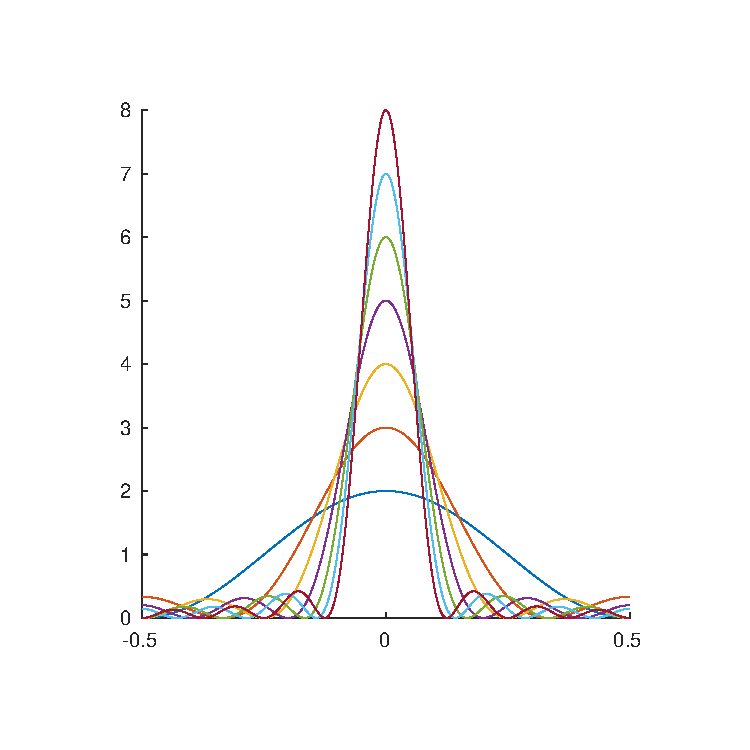
\includegraphics[width = \textwidth]{matlab/fejerkernel}
\caption{Fejer Kernel}
\label{fejer}
\end{figure}
\end{example}

\begin{theorem}
approx. id. on locally compact group G with left Haar measure
\end{theorem}

\begin{theorem}
ke familz of funcs on loc compact group G with properties...
\end{theorem}

\section{Required Stuff}

\begin{enumerate}
\item hausdorf topological space
\item counting measure
\item area of intersecting circles
\item banach algebra
\item hoelders inequality
\item fubini
\item chebyschevs inequality
\item lebesgue dominated conv. thm.
\item measure theoretic support
\end{enumerate}

chapter 1 stuff:
\begin{enumerate}
\item Lp norms and other defs etc.
\item distr. functions
\end{enumerate}

\end{document}